 \documentclass[11pt,a4paper,oneside]{article}


\usepackage{makeidx}  % allows for indexgeneration
\usepackage[dvips]{graphicx}
\usepackage{caption}
\usepackage{subcaption}
\usepackage{dsfont}
\usepackage{amsmath}
\usepackage{algorithm}
\usepackage{algorithmic}
\usepackage{blindtext}
\usepackage{array}

\usepackage{cite}
\usepackage{url}  % Formatting web addresses
%\usepackage{showkeys}
\usepackage{epsfig}
\usepackage{color}
\usepackage{psfrag}

%\usepackage{natbib}
\usepackage[english]{babel}

\usepackage{rotating}
\usepackage{rotate}
\usepackage{lscape}

\usepackage{multirow}

 
\usepackage{graphicx}% Include figure files
\usepackage{dcolumn}% Align table columns on decimal point
\usepackage{bm}% bold math



\def\lim{\mathop{\rm lim}}
\def\argmax{\mathop{\rm argmax}}
\def\argmin{\mathop{\rm argmin}}
\def\sup{\mathop{\rm sup}}

%\nofiles

\makeatletter
\newcommand*{\rom}[1]{\expandafter\@slowromancap\romannumeral #1@}

\begin{document}

\title{Report for assingment 03:\\ ``Bootstrap for gene differential expression analysis of the prostate cancer data''}

\author{Alexey Stupnikov\\
Computational Biology and Machine Learning Laboratory\\ Center for Cancer Research and Cell Biology\\ School of Medicine, Dentistry and Biomedical Sciences\\  Faculty of Medicine, Health and Life Sciences\\ Queen's University Belfast\\ 97 Lisburn Road, Belfast, BT9 7BL, UK, \texttt astupnikov01@qub.ac.uk
}

\date{12.11.2013}
\maketitle

\newpage
\setcounter{secnumdepth}{1}

\section{Summary}

This report describes the bootstrap results for gene differential expression analysis performed under various sampling and adjustment techniques.




\section{Aims and Objectives}


Using Affymetrix gene expression data achieved in \cite{singh2002gene} explore the influence of sample size and adjustment technique on the gene differential expression results. 




\section{Methods}

Data used in this assignment consists of 52 \emph{normal} and 50 \emph{tumour} samples.
RMA was used for data preprocessing and normalisation. Then, expression matrix was processed to unite probesets corresponding to the same genes in order to implement \emph{``genewise''} analysis instead of \emph{``probewise''}. This also allowed to reduce the amount of hypothesises. 
After that bootstrap in two variations was performed. In the first approach, 20 samples from all samples pool of the same condition(normal/tumour) were selected randomly without replacement (randomisation was done by using standard R functions). Second approach involved random selection of 50 samples with replacement from same pools.
Two obtained sample arrays were analysed for differential expression. Significance level was considered $p-value \leq 0.05$. Different multiple hypothesises testing adjustments were used: Bonferroni and less strict Benjamini-Hochberg FDR rate. Combined to 2 bootstrap variations it gives 4 different cases to compare.




\section{Results}

The results are introduced in a form of histograms. The horizontal axis represents the amount of significant genes found in a bootstrap iteration. The vertical axis represents the amount of iterations where such amount was observed.


%\begin{figure}[p]
%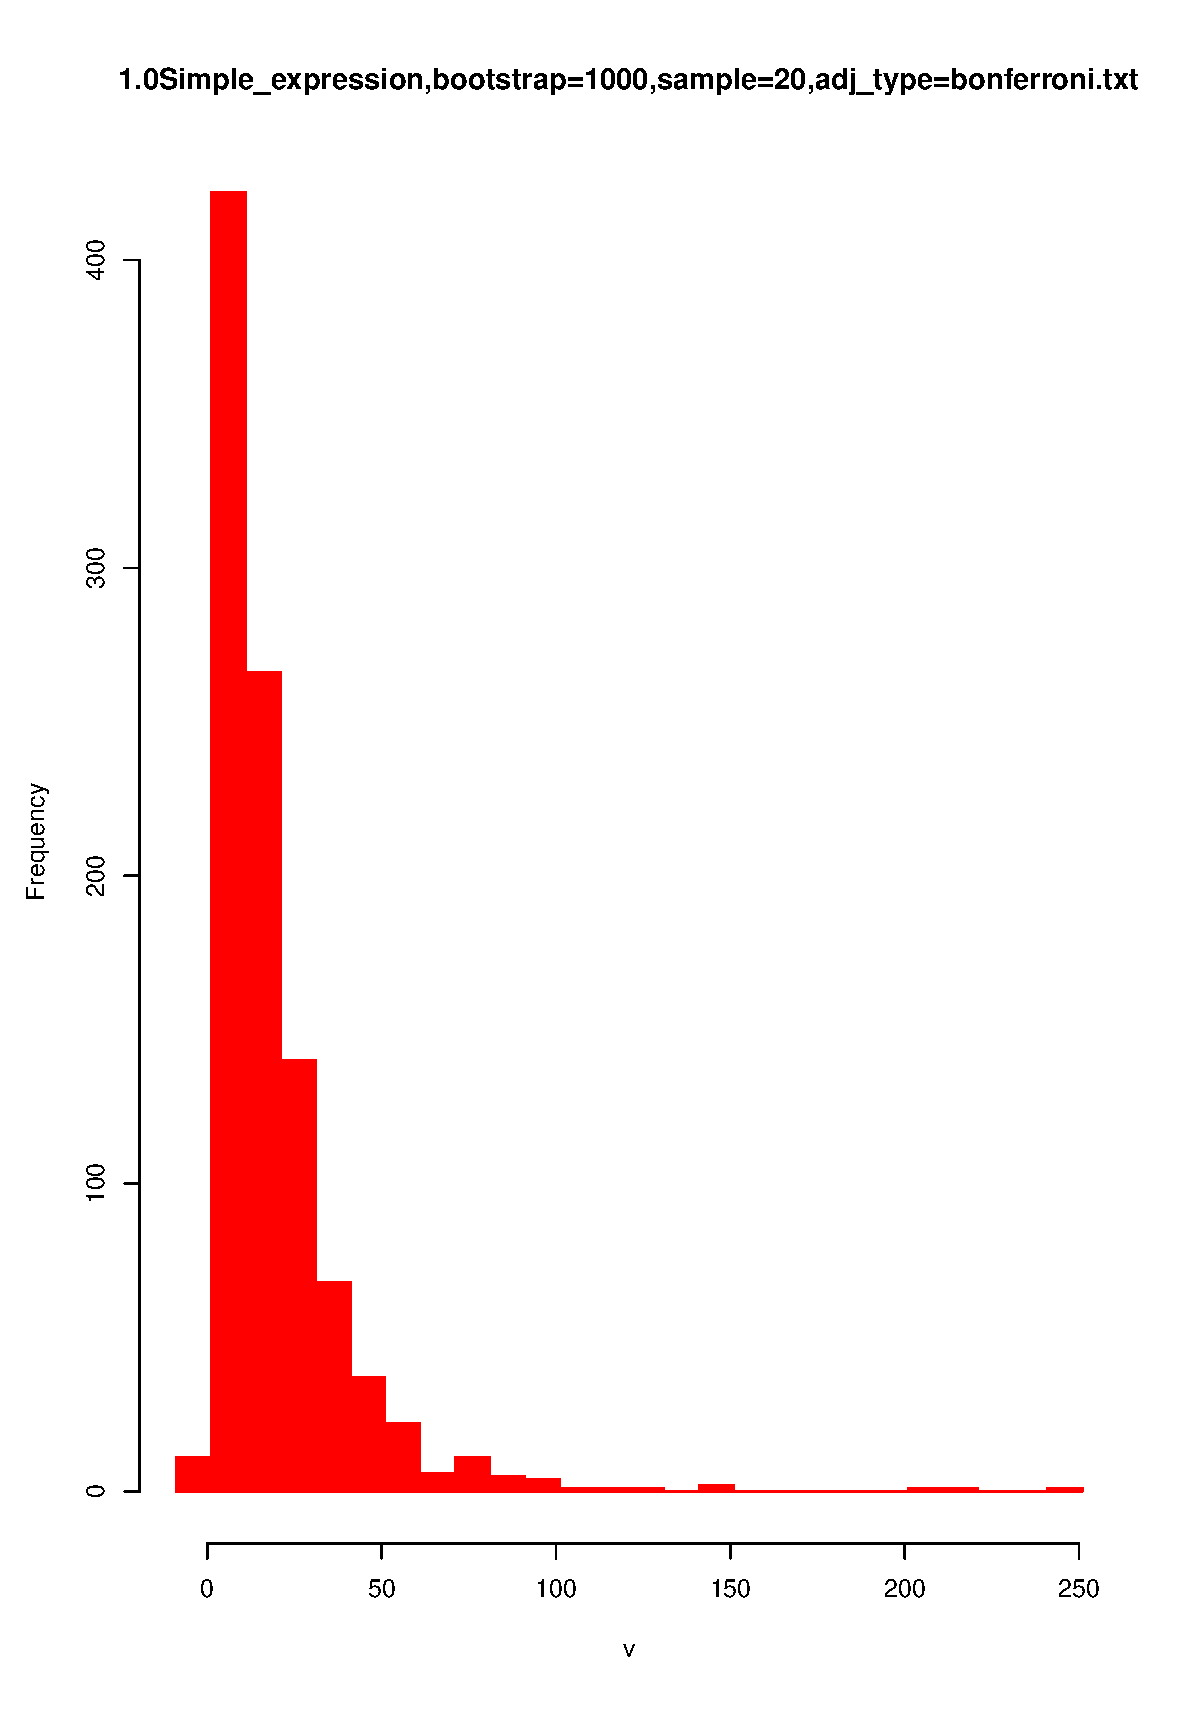
\includegraphics[scale=0.25]{1.0Simple_expression,bootstrap=1000,sample=20,adj_type=bonferroni.txt.eps}
%\caption{Significant genes amounts achieved in bootstrap inerations\\Bootstrap %sample size 20\\Adjustment method Bonferroni}\label{fig:pm1}
%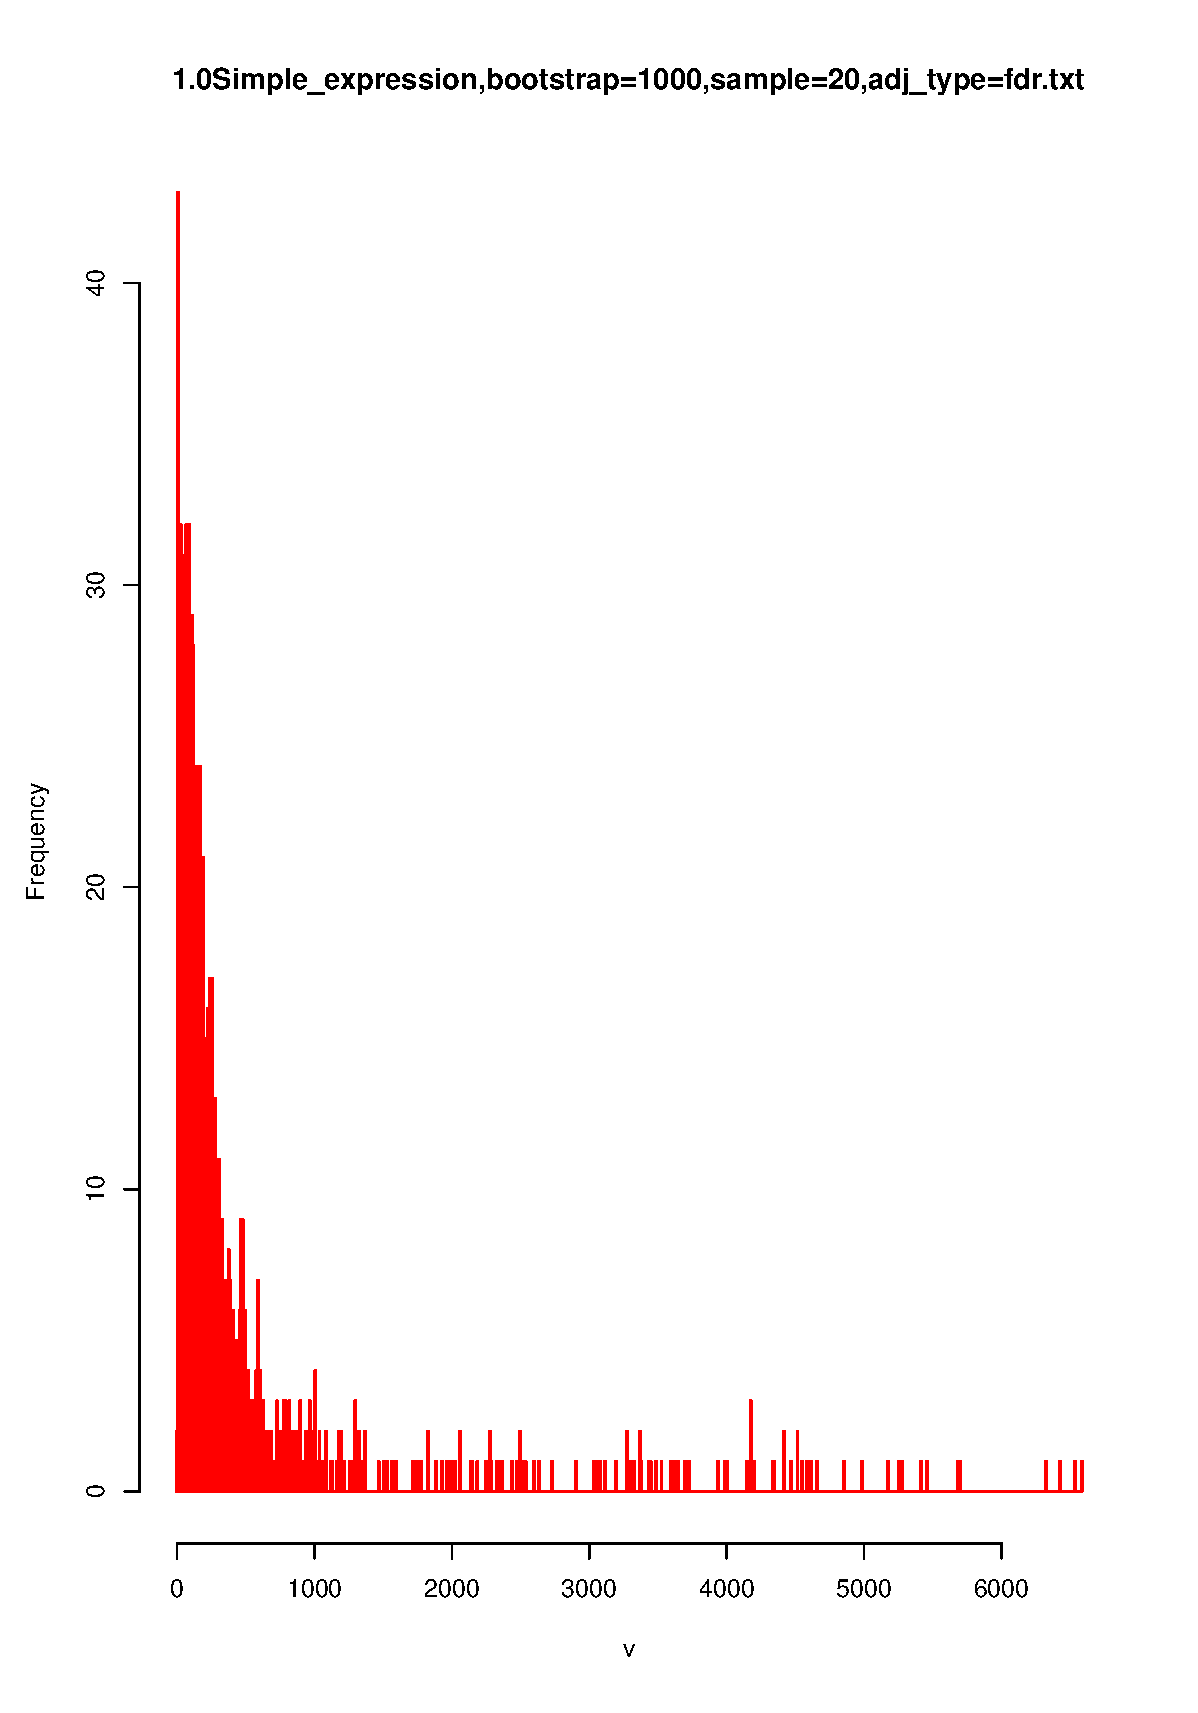
\includegraphics[scale=0.25]{1.0Simple_expression,bootstrap=1000,sample=20,adj_type=fdr.txt.eps}
%\caption{Significant genes amounts achieved in bootstrap inerations\\Bootstrap sample size 20\\Adjustment method Benjamini?Hochberg}\label{fig:pm2}
%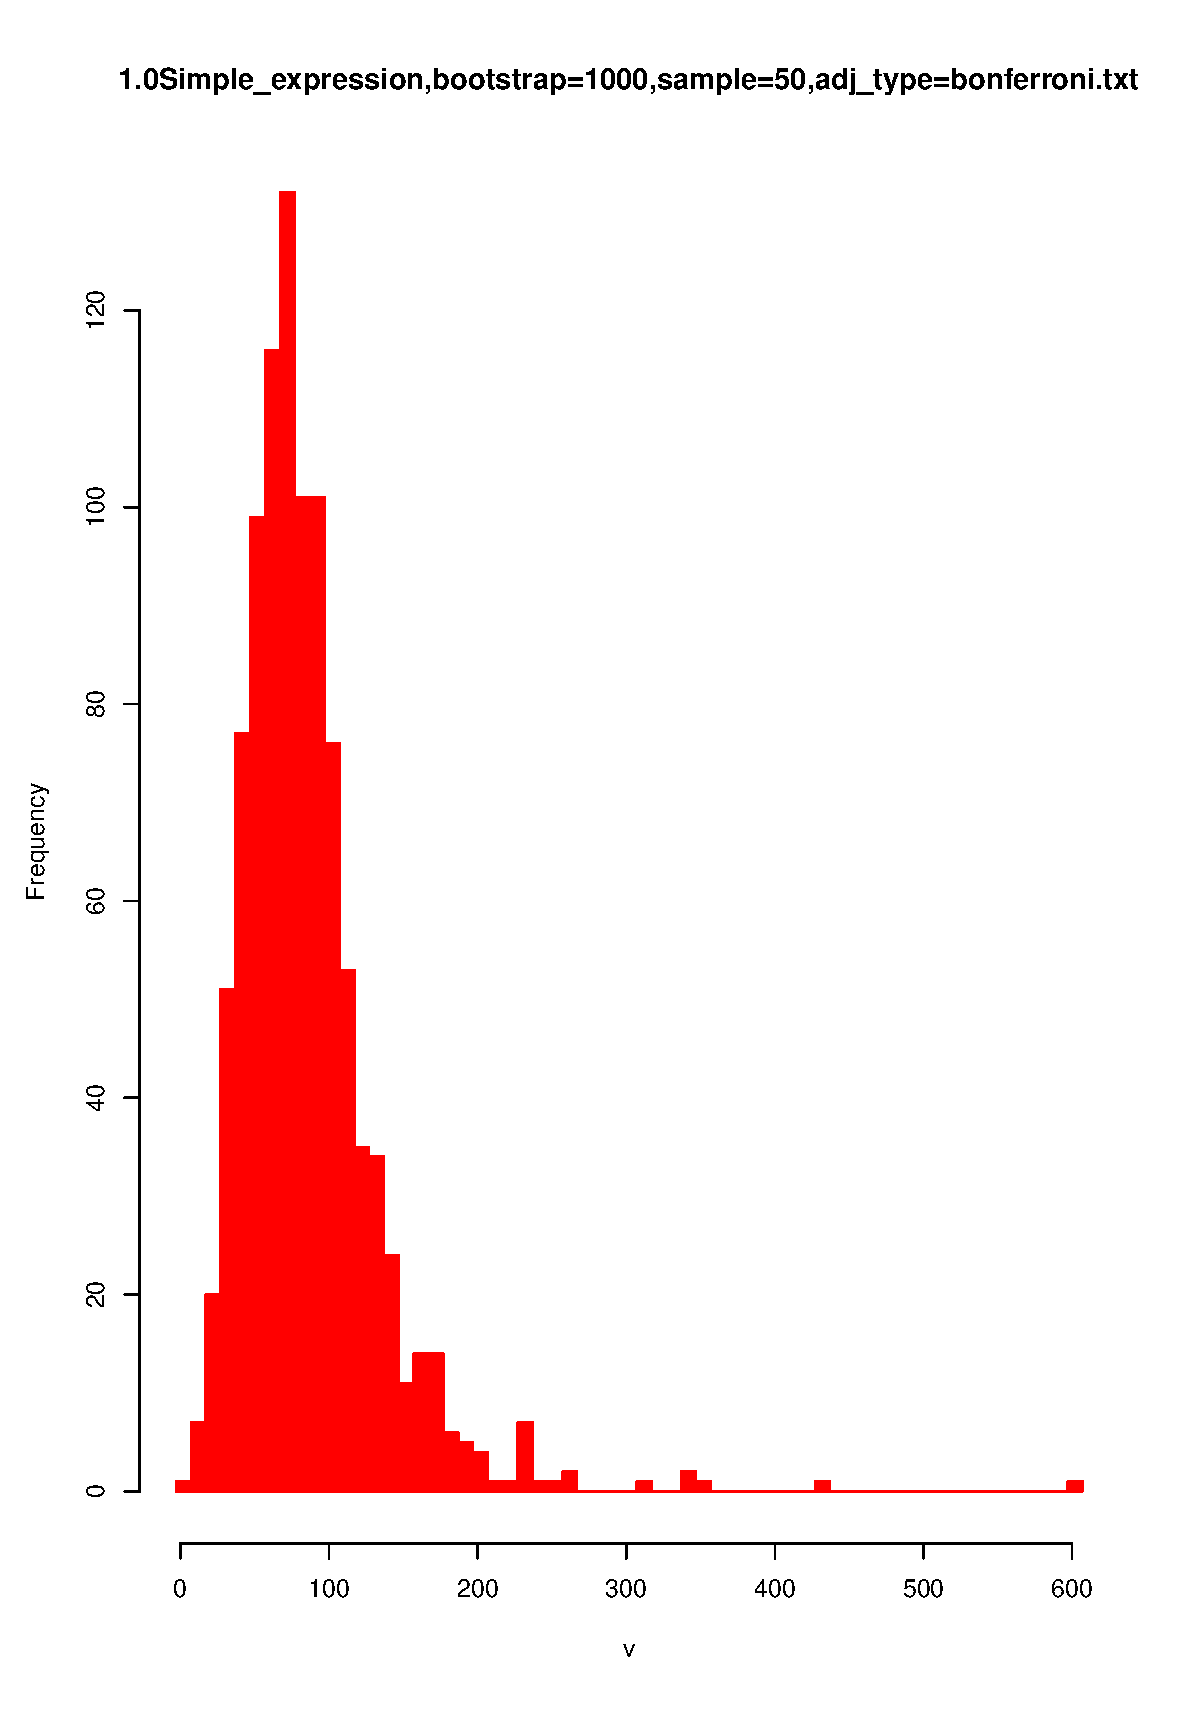
\includegraphics[scale=0.25]{1.0Simple_expression,bootstrap=1000,sample=50,adj_type=bonferroni.txt.eps}
%\caption{Significant genes amounts achieved in bootstrap inerations\\Bootstrap sample size 50\\Adjustment method Bonferroni}\label{fig:pm3}
%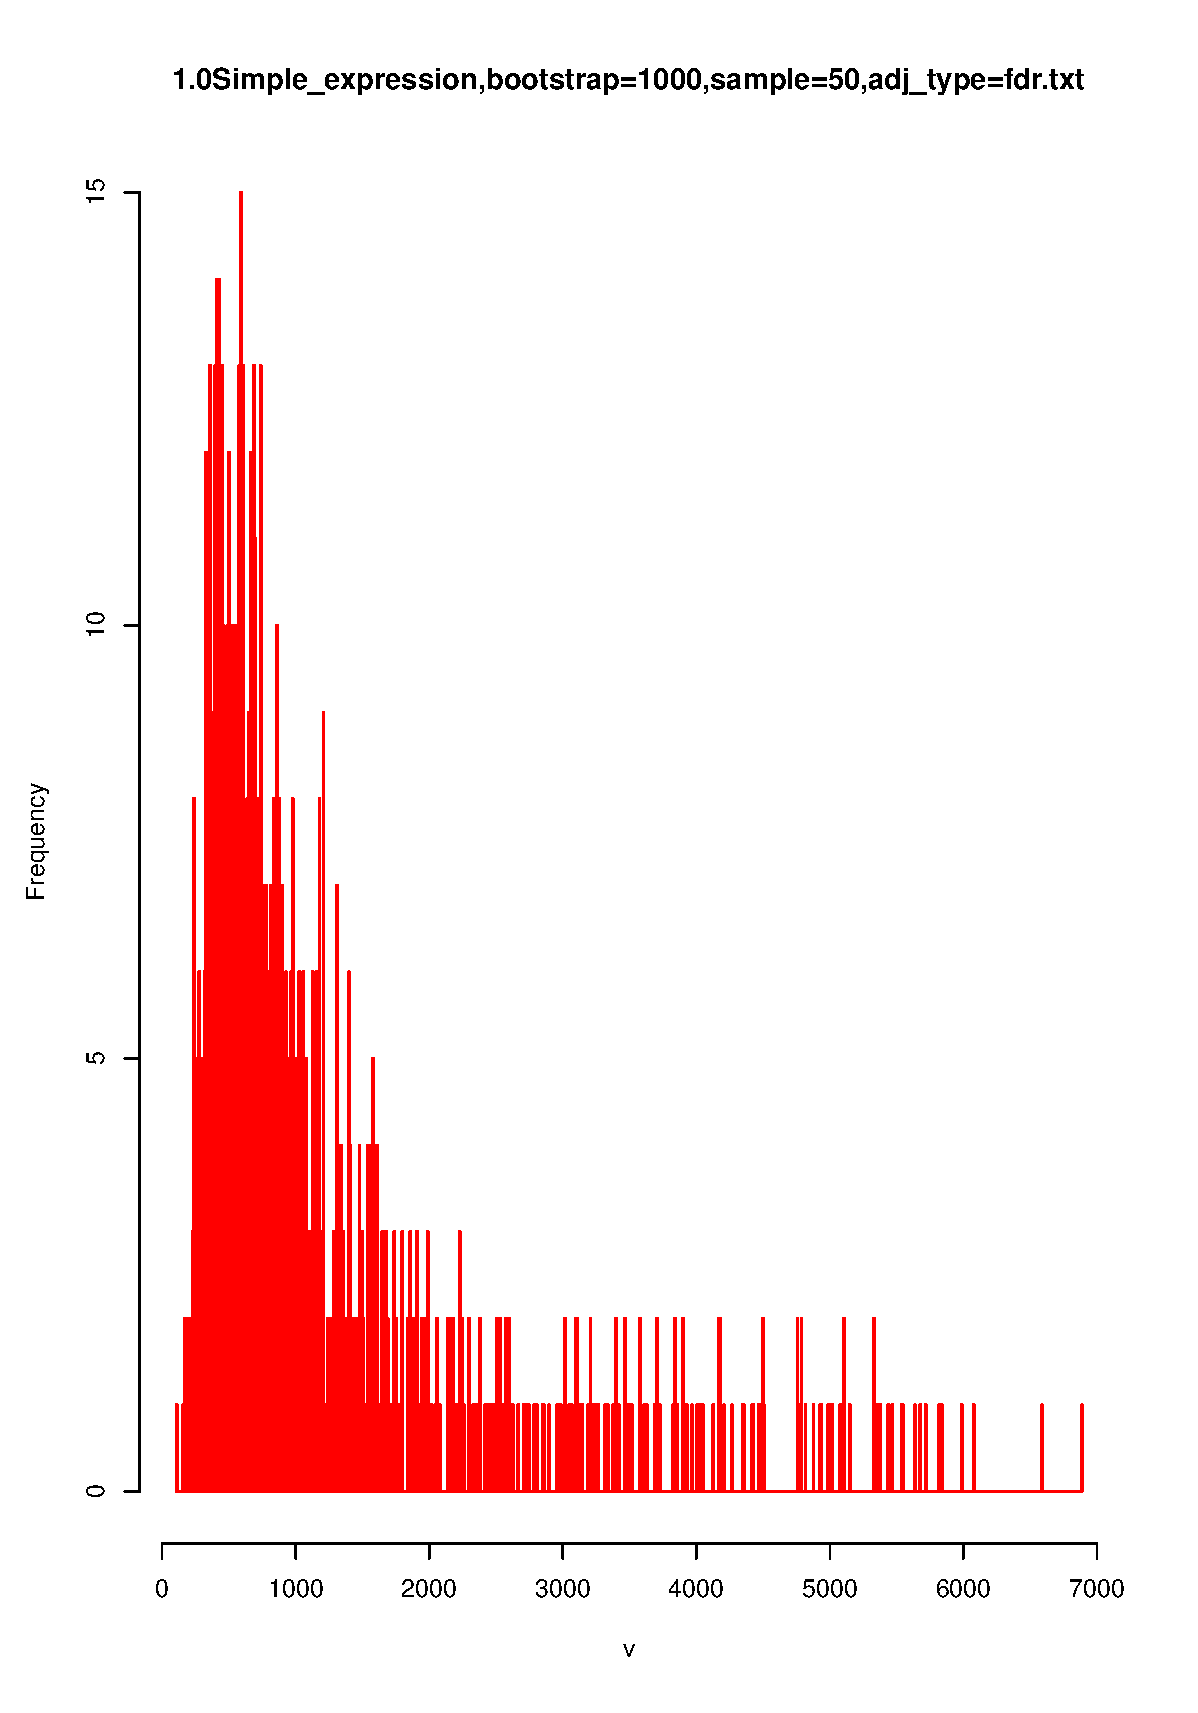
\includegraphics[scale=0.25]{1.0Simple_expression,bootstrap=1000,sample=50,adj_type=fdr.txt.eps}
%\caption{Significant genes amounts achieved in bootstrap inerations\\Bootstrap sample size 50\\Adjustment method Benjamini?Hochberg}\label{fig:pm4}

%caption{main caption}\label{all_figures}
%\end{figure}


\begin{figure}
\centering
\begin{subfigure}[b]{0.4\textwidth}
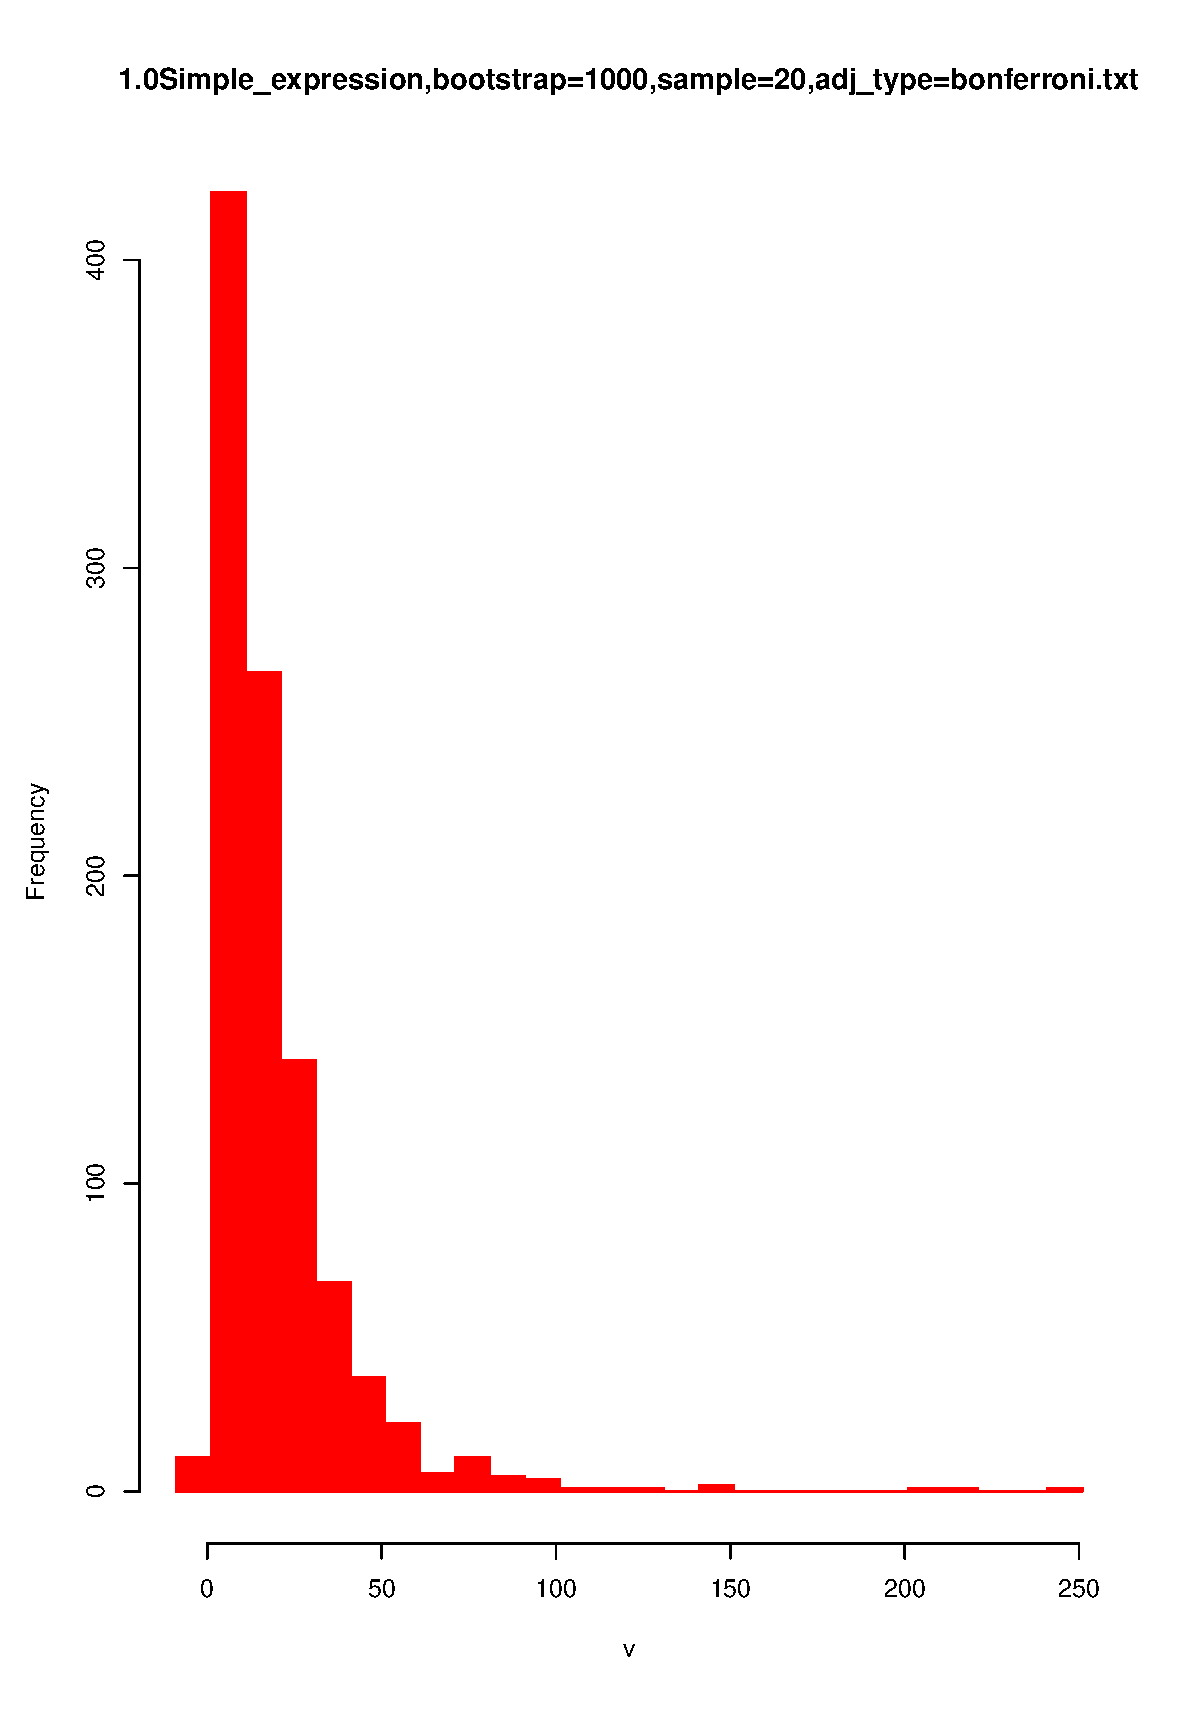
\includegraphics[width=\textwidth]{1.0Simple_expression,bootstrap=1000,sample=20,adj_type=bonferroni.txt.eps}
\caption{Bootstrap sample size 20\\Adjustment method Bonferroni}
\label{fig:pm1}
\end{subfigure}%
~~~~~~~~~~~~
\begin{subfigure}[b]{0.4\textwidth}
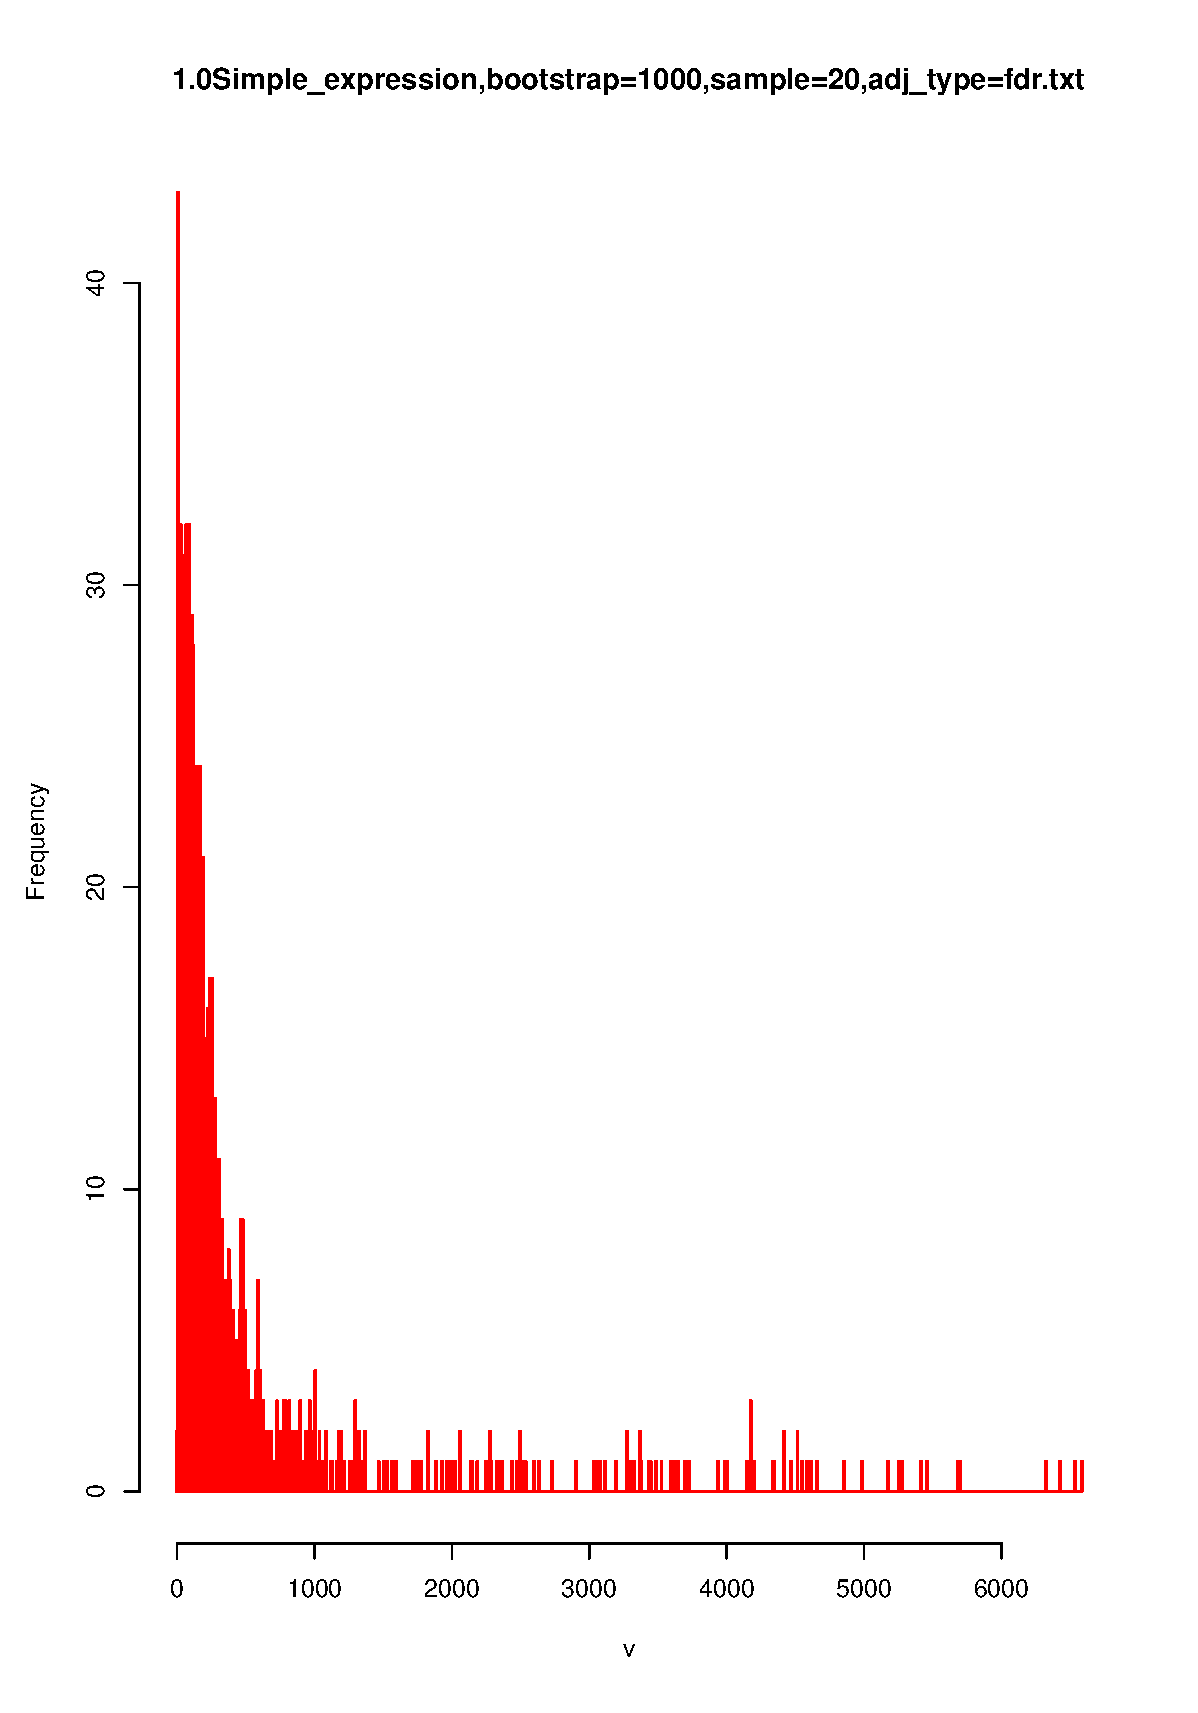
\includegraphics[width=\textwidth]{1.0Simple_expression,bootstrap=1000,sample=20,adj_type=fdr.txt.eps}
\caption{Bootstrap sample size 20\\Adjustment method Benjamini-Hochberg}
\label{fig:pm2}
\end{subfigure}
\\
\begin{subfigure}[b]{0.4\textwidth}
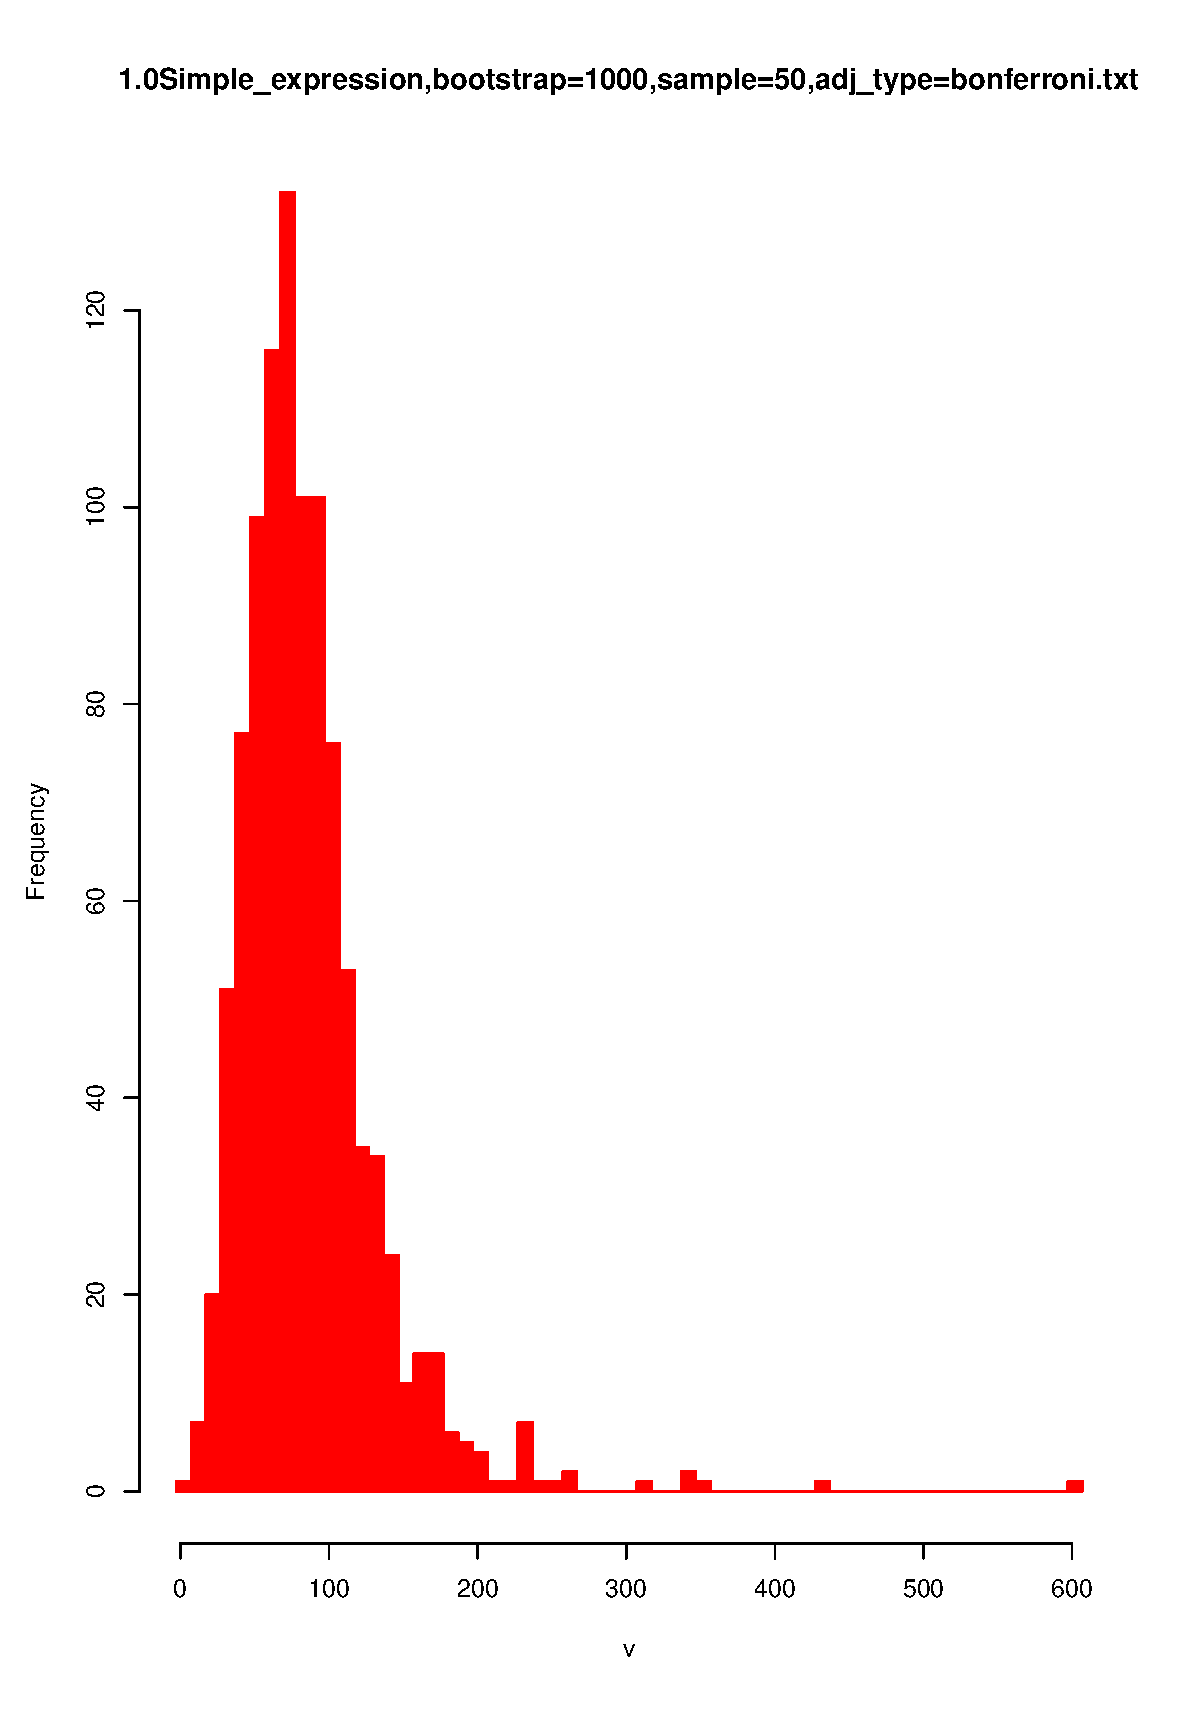
\includegraphics[width=\textwidth]{1.0Simple_expression,bootstrap=1000,sample=50,adj_type=bonferroni.txt.eps}
\caption{Bootstrap sample size 50\\Adjustment method Bonferroni}
\label{fig:pm3}
\end{subfigure}
~~~~~~~~~~~~
\begin{subfigure}[b]{0.4\textwidth}
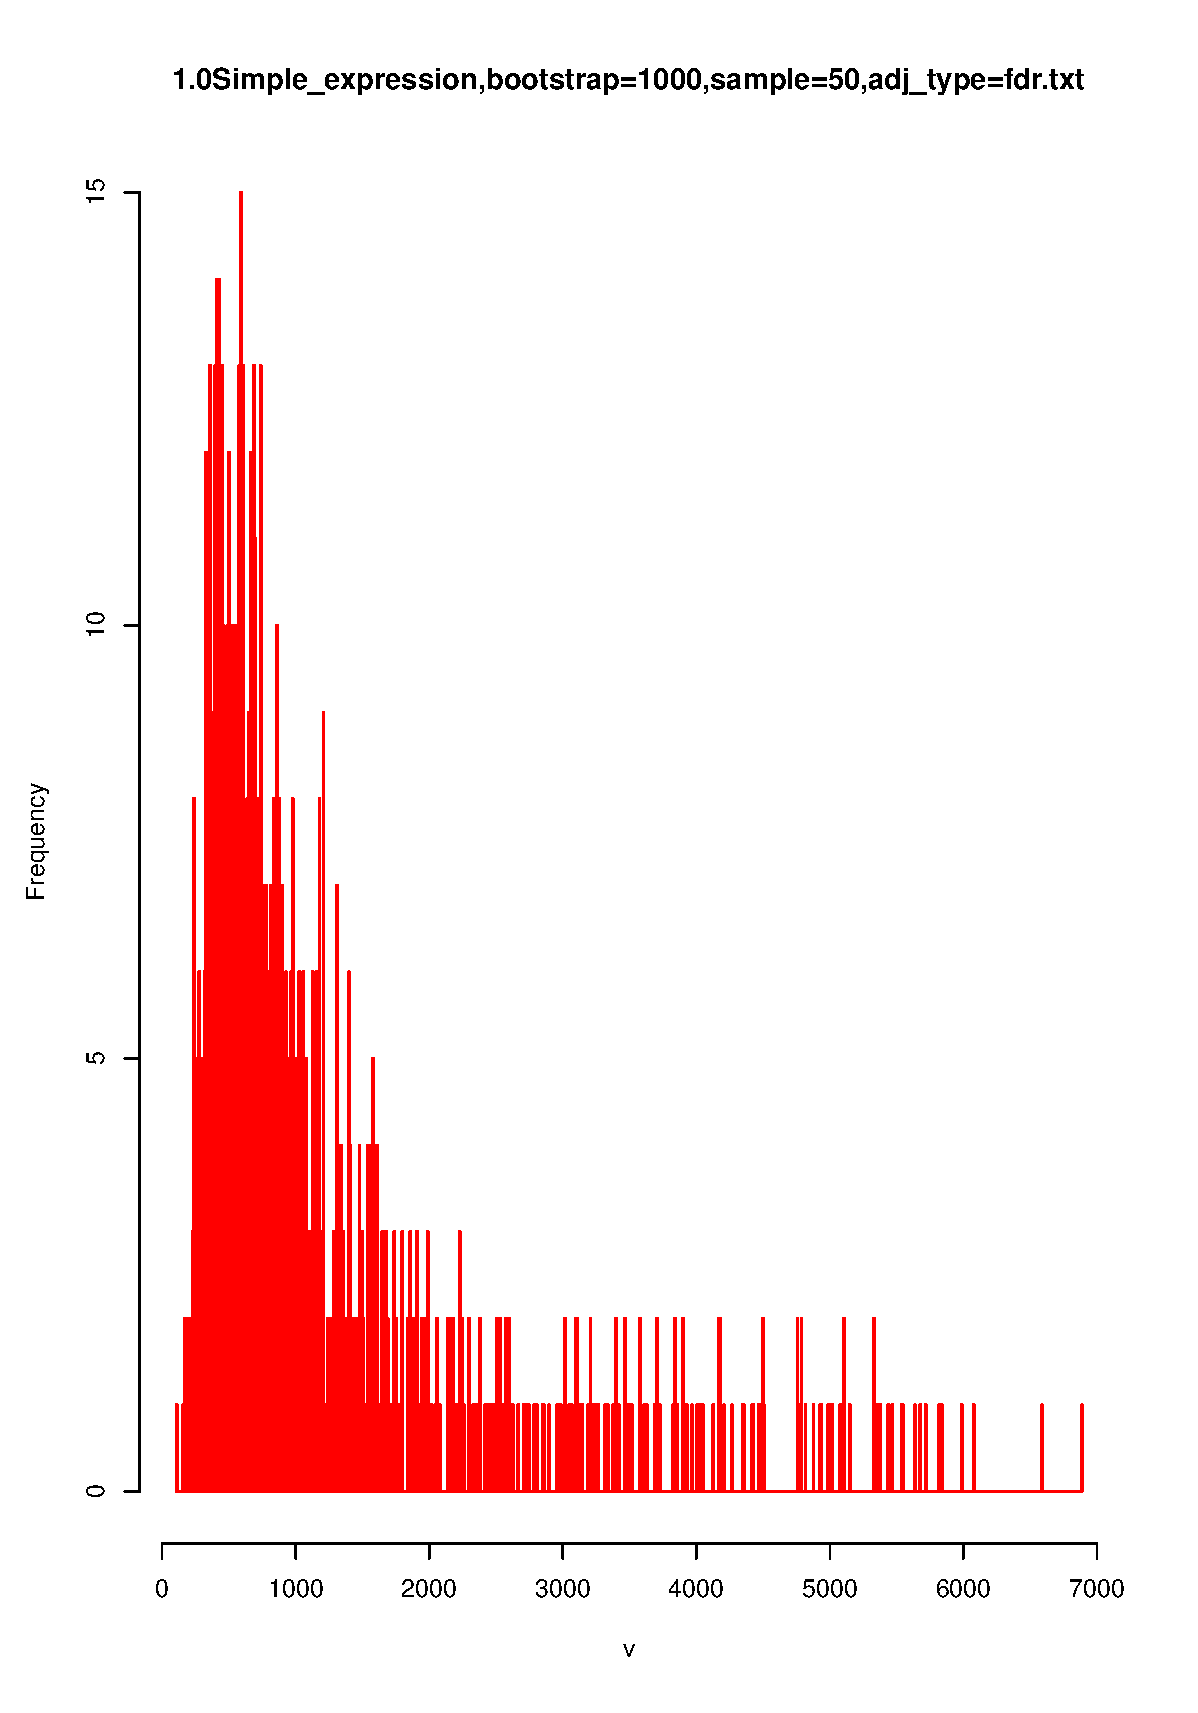
\includegraphics[width=\textwidth]{1.0Simple_expression,bootstrap=1000,sample=50,adj_type=fdr.txt.eps}
\caption{Bootstrap sample size 50\\Adjustment method Benjamini-Hochberg}
\label{fig:pm4}
\end{subfigure}
\caption{Significant genes amounts achieved in bootstrap inerations}\label{fig:allfigures}
\end{figure}


\section{Conclusion}

From the histograms it is clear that the amount of samples, as well as adjustment technique used for differential expression analysis has a drastic impact on the result.
Bonferroni adjustment method excludes many significant genes, whereas Benjamini-Hochberg method allows to obtain much more significant genes. However, fdr method does not exclude certain unprobable from practical point of view cases with amount of significant genes of 7000.
Bootstrap with sample size 20 gives much less significant genes than one with the size of 50.
In a regular non-bootstrap analysis involving all samples, there were discovered 2263 significant genes and 7457 non-significant. 

  


%\bibliographystyle{cell}
\bibliographystyle{plain}
\bibliography{/home/alex/B/Stud/03/Report/Report.bib}
%,/Users/fes/Local/Mails/CV/Bibref/bib_ref_journals,/Users/fes/Local/Mails/CV/Bibref/bib_ref_books_editor}     % Bibliography file (usually '*.bib' )


%\newpage

%\section*{Figure Legends}






\end{document}
%
% ****** End of file apssamp.tex ******
